\clearpage
{\bfseries SRSTI 50.47.00:20.23.19}\hfill
\hfill {\bfseries \href{https://doi.org/10.58805/kazutb.v.2.19-96}{https://doi.org/10.58805/kazutb.v.2.19-96}}

\sectionwithauthors{Akishev K.M., Karpov V.I., Akisheva L., Tulegulov А.D.}{DATAMINING CAPABILITIES FOR CLUSTERING CONCRETE MIX
FORMULATIONS}

\begin{center}
{\bfseries K.M. Akishev\textsuperscript{1*},V.I. Karpov\textsuperscript{2},
L.A. Akisheva\textsuperscript{3}, A.D.Tulegulov\textsuperscript{1}}

\textsuperscript{1}Kazhach University of Technology and
Business,

\textsuperscript{2}Moscow State University of Technology and
Management named after K.G. Razumovsky,

\textsuperscript{3}Nazarbayev
Intellectual School

e-mail: Akmail04cx@mail.ru
\end{center}

The article discusses the possibilities of using DataMining technology
for clustering concrete mixtures. In practice, it is often necessary to
face tasks in which it is necessary to choose the formulations closest
in quality characteristics from a large number of formulations of
concrete mixtures. The distribution of formulations of concrete mixtures
by classes is provided on the basis of specified criteria such as
strength, as well as the composition of the ingredients of the concrete
mixture. Earlier in work {[}1{]}, clustering of concrete mix
formulations was carried out with the help of the program "Comprehensive
quality assessment and classification of multidimensional objects",
which made it possible to distribute formulations into classes with the
closest characteristics and collect the highest quality concrete mix
formulations into the appropriate classes. The result of using
DataMining technology for clustering concrete mix formulations allowed
us to create classes in which the distribution using the DBSCAN
algorithm is quite high-quality, however, there is a need for more
detailed training of this algorithm, since clustering using the program
"Integrated Quality Assessment and classification of multidimensional
objects" turned out to be more optimal.

{\bfseries Keywords} : clustering, datamining, concrete mix formulations,
quality criteria

\begin{center}
{\large\bfseries БЕТОН ҚОСПАЛАРЫНЫҢ РЕЦЕПТЕРІН КЛАСТЕРЛЕУГЕ АРНАЛҒАН DATA MINING
МҮМКІНДІКТЕРІ}

\vspace{1em}
{\bfseries К.М.Акишев\textsuperscript{1*}, В.И.Карпов\textsuperscript{2},
Л.Ақышева\textsuperscript{3}, А.Д.Тулеғулов\textsuperscript{1}}

\textsuperscript{1}Қазақ технология және бизнес университеті,

\textsuperscript{2} К. Г. Разумовский атындағы Москеу мемлекеттік
технология және басқару университеті

\textsuperscript{3} Назарбаев Зияткерлік мектебі,

e-mail: Akmail04cx@mail.ru
\end{center}

Мақалада бетон қоспаларын кластерлеу үшін DataMining технологиясын
қолдану мүмкіндіктері қарастырылады. Іс жүзінде сіз көбінесе бетон
қоспаларының көптеген рецептерінен сапалық сипаттамалары бойынша ең
жақын рецептілерді таңдау қажет болатын міндеттерге тап болуыңыз керек.
Бетон қоспаларының рецептураларын сыныптар бойынша бөлу беріктік,
сондай-ақ бетон қоспасының ингредиенттерінің құрамы сияқты берілген
критерийлер негізінде қамтамасыз етіледі. {[}1{]} -жұмыстың басында
бетон қоспаларының рецептураларын кластерлеу "сапаны кешенді бағалау
және көпөлшемді объектілерді жіктеу" бағдарламасының көмегімен жүзеге
асырылды, бұл рецептураларды ең жақын сипаттамалары бар сыныптарға
бөлуге және бетон қоспаларының ең сапалы рецептураларын тиісті
сыныптарға жинауға мүмкіндік берді. Бетон қоспаларының формулаларын
кластерлеу үшін DataMining технологиясын қолданудың нәтижесі DBSCAN
алгоритмін қолдана отырып бөлу өте сапалы болатын сыныптар құруға
мүмкіндік берді, дегенмен бұл алгоритмді егжей-тегжейлі оқыту қажет,
өйткені "сапаны кешенді бағалау және көп өлшемді объектілерді жіктеу"
бағдарламасын қолдана отырып кластерлеу оңтайлы болды.

{\bfseries Түйін сөздер}: кластерлеу, datamining, бетон қоспаларының
формулалары, сапа критерийлері.

\newpage
\begin{center}
{\large\bfseries ВОЗМОЖНОСТИ DATAMINING ДЛЯ КЛАСТЕРИЗАЦИИ РЕЦЕПТУР БЕТОННЫХ
СМЕСЕЙ}

\vspace{1em}
{\bfseries К.М.Акишев\textsuperscript{1*}, В.И.Карпов\textsuperscript{2},
Л.Акишева\textsuperscript{1}, А.Д.Тулегулов\textsuperscript{1}}

\textsuperscript{1}Казахский университет технологии и бизнеса,

\textsuperscript{2}Московский Государственный университет
технологии и управления им. К.Г. Разумовского,

\textsuperscript{3}Назарбаев интеллектуальная школа,

e-mail: Akmail04cx@mail.ru
\end{center}

В статье рассматривается возможности использования технологии DataMining
для кластеризации бетонных смесей. На практике часто приходится
сталкиваться с задачами в которых необходимо из большого количества
рецептур бетонных смесей выбрать наиболее близкие по качественным
характеристикам рецептуры. Распределение рецептур бетонных смесей по
классам обеспечивается на основании заданных критериев таки, как
прочность, а также состав ингредиентов бетонной смеси. Раннее в работе
{[}1{]}, кластеризация рецептур бетонных смесей была осуществлена с
помощью программы «Комплексная оценка качества и классификация
многомерных объектов», позволившая распределить рецептуры по классам с
наиболее близкими характеристиками и собрать наиболее качественные
рецептуры бетонных смесей в соответствующие классы. Результат
использования технологии DataMining для кластеризации рецептур бетонных
смесей позволил создать классы в которых распределение c помощью
алгоритма DBSCAN достаточно качественно, тем не менее существует
необходимость более детального обучения данного алгоритма, так как
кластеризация с использованием программы «Комплексная оценка качества и
классификация многомерных объектов» оказалось более оптимальной.

{\bfseries Ключевые слова}: кластеризация, datamining, рецептуры бетонных
смесей, критерии качества

\vspace{0.5em}

\begin{multicols}{2}
{\bfseries Introduction.}To date, the active promotion of information
technology (datamining) provides the necessary and sufficient
opportunities to obtain reliable and high-quality results, in particular
for solving clustering and forecasting problems.

Data analysis depends on efficient data collection, storage and computer
processing. Data Mining allows you to analyze large volumes of
heterogeneous data of various scientific fields.

The international market of DataMining systems has a dynamic growth.
Firms such as SAS, IBM, Microsoft, Oracle, provide investments of \$56.2
billion by 2027 {[}2{]}.

Promising trends in DataMining allow us to develop methods of virtual
and augmented reality analysis, statistical data analysis, and data
protection.

It is known for certain that data mining in the future for big data
analysis using corporate databases.

At the same time, the main criterion for DataMining technology is the
system time required to complete the tasks. At the same time, the main
difficulty lies in the limitations that arise during the search of
decision trees, which affect the efficiency and performance of the
search.

Solving this problem remains the main goal of DataMining product
developers{[}2{]}.

When performing clustering tasks, there are a number of typical,
standard stages for DataMining, which include:

-statement of the task, which includes the analysis of requirements, the
definition of the problem area, the metrics for which the assessment
will be performed, as well as the definition of tasks for the analysis
project;

-preparation of data, evaluation criteria;

-research and evaluation of data;

-building analytical dependencies;

-research, verification of the accuracy of solutions.

Today, everyone who deals with problems in the field of big data
processing must have skills in the field of mathematical statistics,
programming languages, machine learning techniques, statistical
analysis, predictive decisions, including managerial decision-making,
depend on the accuracy and in-depth data analysis.

To date, there is a wide selection of programs on the market for solving
Data Mining problems. Let\textquotesingle s look at the main ones:

SAS EnterpriseMiner - used mainly for fraud detection, financial risk
assessment, market forecasting, etc. It has a fairly high performance
when working with big data;

-MicrosoftAnalysisServices - used to create analytical reports;

-SAS CustomerIntelligence 360 - used as a tool for information
business, evaluation of marketing campaigns, real-time data analysis;

-SAS CreditScoring - used as a risk management tool for financial
institutions;

-Board - nothing remarkable, for business analytics, corporate
governance, evaluation of the effectiveness of projects.

-SAS RevenueOptimization - a use case as an intellectual business
tool, mainly in retail;

-RapidMiner - is used for text analysis, machine learning, and the
creation of analytical reports.

{\bfseries The aim of the study} is to evaluate the DataMining technology
for clustering concrete mix formulations and compare the results with
the data obtained using the program "Comprehensive quality assessment
and classification of multidimensional objects" with the possibility of
using DataMining technology in further studies of clustering problems of
technogenic deposits.

In {[}1{]}, prior to the start of cluster analysis, each object under
study or the formulation of a concrete mixture is a separate cluster,
and the proximity between clusters is assumed by accepted metrics.

The most optimal way to solve the research problem, determining
proximity (distances) between clusters in the studied space, or as they
say in many sources, Euclidean distances. "Euclidean distance is a
general type of distance used from ancient times to the present day, it
is a geometric distance in multidimensional space"{[}3{]} and is used in
various methods.

As a result of the solution {[}1{]}, a mathematical formulation of the
problem of clustering concrete mixtures using technogenic waste formula
1 was obtained.

\begin{equation}
F(C_k, C_l) = \frac{1}{{N_k \cdot N_l}} \sum\limits_{SiCk} \sum\limits_{SjCl} f(S_j, S_j)
\end{equation}

That is, each cluster contains formulations of concrete mixtures that
are closest in their characteristics and the formulations of each class
differ from each other.

For the software implementation of the mathematical formulation of the
solution of the problem of clustering concrete mixtures, the program
"Comprehensive quality assessment and classification of multidimensional
objects" in Russian was used. Data on the metrics of the recipe of
concrete mixtures are presented in Table 1.
\end{multicols}

\begin{longtable}[]{@{}
  |>{\raggedright\arraybackslash}p{(\columnwidth - 8\tabcolsep) * \real{0.1697}}|
  >{\raggedright\arraybackslash}p{(\columnwidth - 8\tabcolsep) * \real{0.1510}}|
  >{\raggedright\arraybackslash}p{(\columnwidth - 8\tabcolsep) * \real{0.1322}}|
  >{\raggedright\arraybackslash}p{(\columnwidth - 8\tabcolsep) * \real{0.1321}}|
  >{\raggedright\arraybackslash}p{(\columnwidth - 8\tabcolsep) * \real{0.4151}}@{}|}
\caption*{Table 1. Recipe of concrete mixtures} \\
\toprule\noalign{}
\multirow{2}{*}{№ recipes} &
\multicolumn{4}{c}{Composition of the concrete mix} \\
& \begin{minipage}[b]{\linewidth}\centering
Ravr. Compr.Mpa
\end{minipage} & \begin{minipage}[b]{\linewidth}\centering
ash
g/\%
\end{minipage} & \begin{minipage}[b]{\linewidth}\centering
Metall. Slag g/\%
\end{minipage} & \begin{minipage}[b]{\linewidth}\centering
bauxite sludge
g/\%
\end{minipage} \\
\midrule\noalign{}
\endfirsthead
\endhead
\bottomrule\noalign{}
\endlastfoot

1 & 3.11 & & & 337/3 \\
\hline
2 & 3.7 & & & 505/4 \\
\hline
3 & 8.32 & & & 674/5 \\
\hline
4 & 3.5 & & & 842/7 \\
\hline
5 & 3.6 & & & 1011/8 \\
\hline
6 & 2.84 & & & 944/7 \\
\hline
7 & 2.56 & & & 910/7 \\
\hline
8 & 2.73 & 574/4.4 & & \\
\hline
9 & 2.3 & 246/2 & & 337/3 \\
\hline
10 & 4.4 & 574/4.4 & & \\
\hline
11 & 2.5 & 656/5 & & \\
\hline
12 & 4.5 & 3370/26 & & \\
\hline
13 & 2.51 & 492/4 & & \\
\hline
14 & 2.8 & 574/4.4 & & \\
\hline
15 & 3.45 & & & 410/3.2 \\
\hline
16 & 4.54 & & & 410,3.2 \\
\hline
17 & 3.9 & 246/2 & 798/6 & \\
\hline
18 & 2.55 & 328/2.5 & 798/6\% & \\
\hline
19 & 3.5 & 328/2.5 & 640/5 & \\
\hline
20-\textsubscript{15} & 1.47 & 107/1.3 & 1066/13 & \\
\hline
21 & 9.74 & 328/2.5 & 798//6 & 246/2 \\
\hline
22 & 3.18 & & 399/3 & 328/2.5 \\
\hline
23 & 3.23 & 164/1.3 & 798/6 & 164/1.3 \\
\hline
24-\textsubscript{15} & 1.6 & & 1020/12 & 357/4.2 \\
\hline
25 & 4.77 & 328/2.5 & 399/3 & 337/2.5 \\
\hline
26 & 4.33 & 164/1.2 & 798/6 & 337/2.5 \\
\hline
27 & 3.3 & 337/2.5 & 798/6 & 164/1.2 \\
\hline
28 & 9 & 337/2.5 & 798/6 & 505/4 \\
\hline
29 & 10 & 337/2.5 & 1596/12 & \\
\hline
30 & 3.22 & 328/.5 & 798/6 & 674/5.2 \\
\hline
31 & 4.62 & 246/2 & & 505/3.2 \\
\hline
32 & 2.3 & & & 1685/13 \\
\hline
33 & 9.1 & 164/1.3 & & 1685/13 \\
\hline
34 & 8.18 & 164/1.3 & & 2022/16 \\
\hline
35 & 4.37 & 1011/8 & & \\
\hline
36 & 1.35 & 7798/80 & & \\
\hline
37 & 4.43 & 337/1.5 & 798/6 & 674/5.2 \\
\hline
38 & 4.13 & 337/2.5 & 798/6 & 337/2.5 \\
\hline
39 & 22.3 & 505/4 & 1197/9. & 337/2.5 \\
\end{longtable}

\begin{figure}[H]
\centering
\begin{subfigure}[t]{0.45\textwidth}
  \centering
  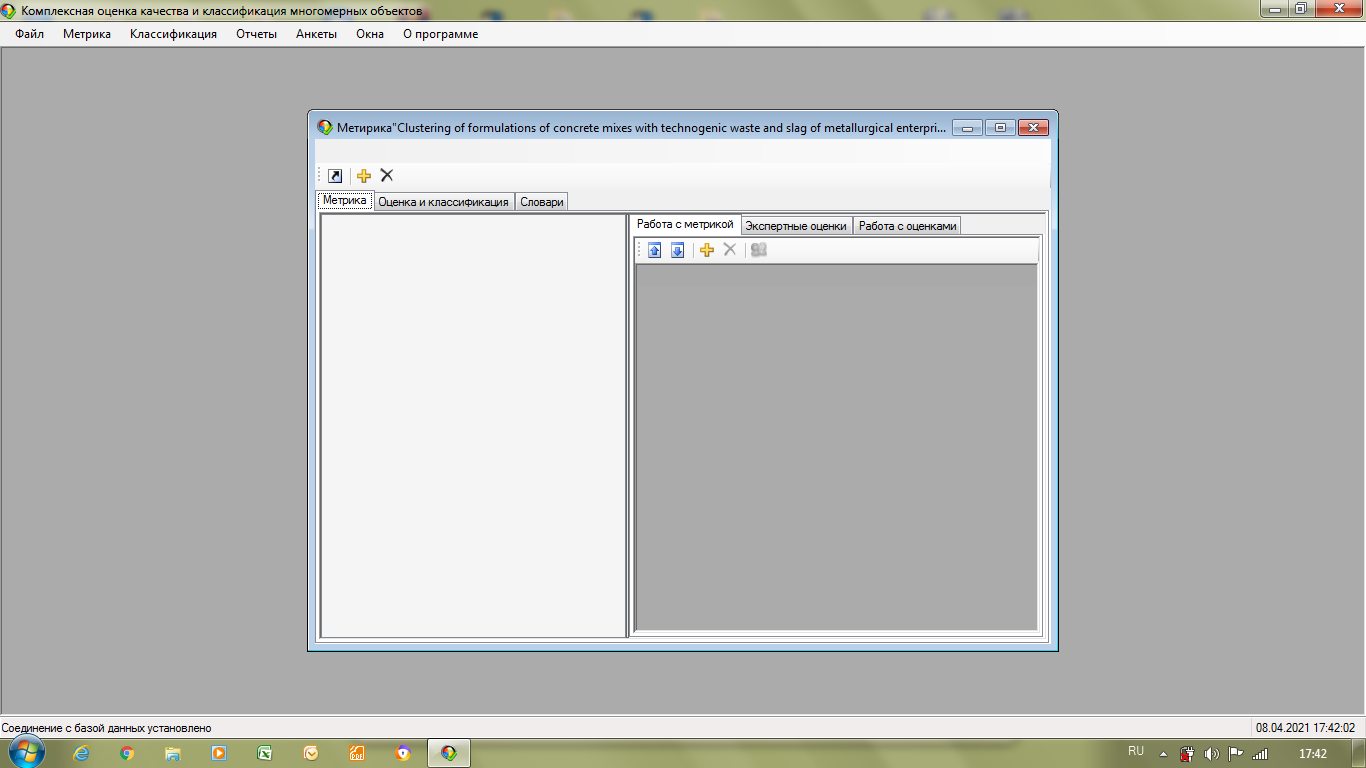
\includegraphics[width=\textwidth]{image8}
  \caption*{Fig. 1- Program interface ""Comprehensive quality assessment and
classification of multidimensional objects"}
\end{subfigure}
\hspace{0.05\textwidth}
\begin{subfigure}[t]{0.45\textwidth}
  \centering
  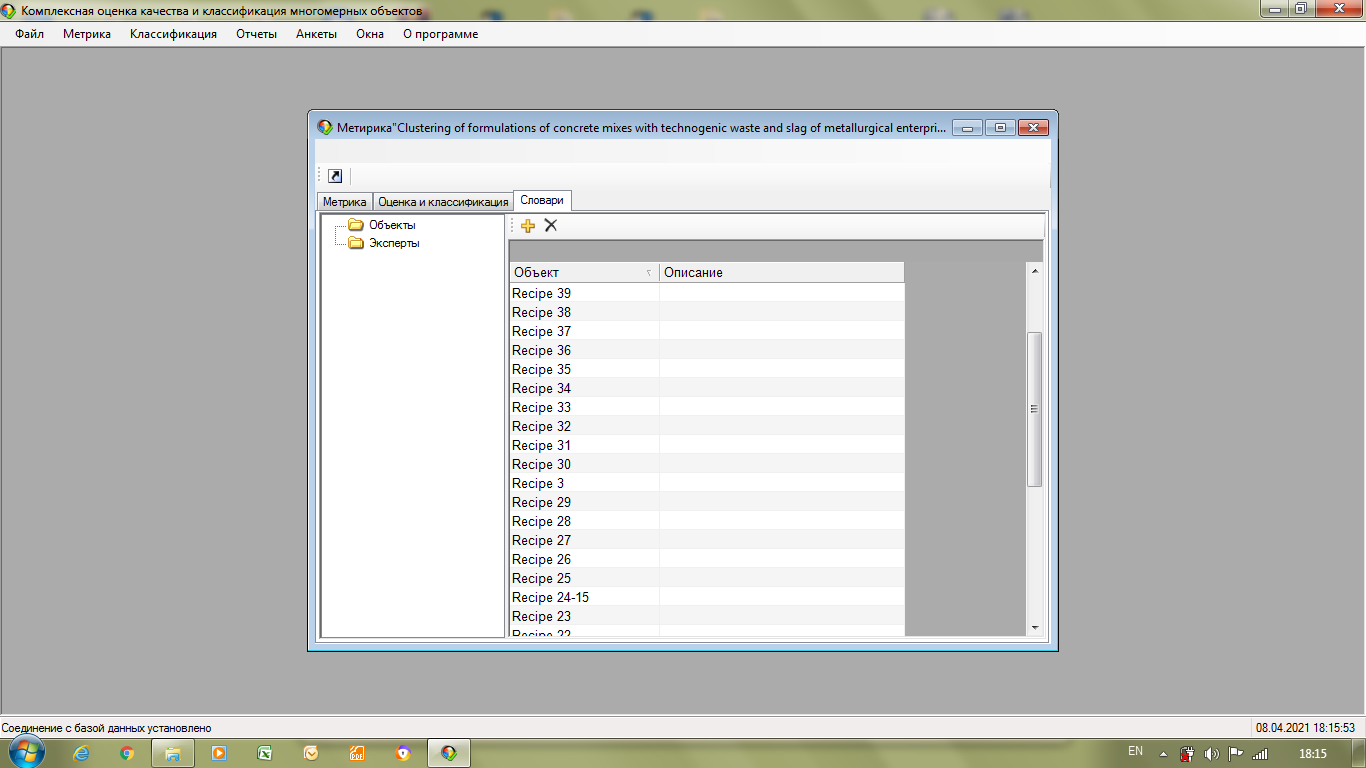
\includegraphics[width=\textwidth]{image9}
  \caption*{Fig. 2 - Shows the input of metrics for compounding concrete mixtures}
\end{subfigure}
\end{figure}

\begin{multicols}{2}
Fig.1-Shows the interface of the program "Comprehensive quality
assessment and classification of multidimensional objects". The data is
entered directly from the keyboard{\bfseries .}

As a result of the program, the distribution of formulations of concrete
mixtures of Table 1, Figure 3 was obtained. In each cluster there are
recipes that are closest in terms of metrics.

From the clustering result obtained, it can be seen that the
formulations of concrete mixtures are distributed in 6 clusters. In each
cluster there are formulations of concrete mixtures with the closest
characteristics in composition and strength. The formulations of
concrete mixtures with low strength indicators are located in clusters
1-4. Table 2 shows the formulations, the composition of concrete
mixtures with the highest strength indicators of 5 and 6 clusters.
\end{multicols}

\begin{figure}
  \centering
  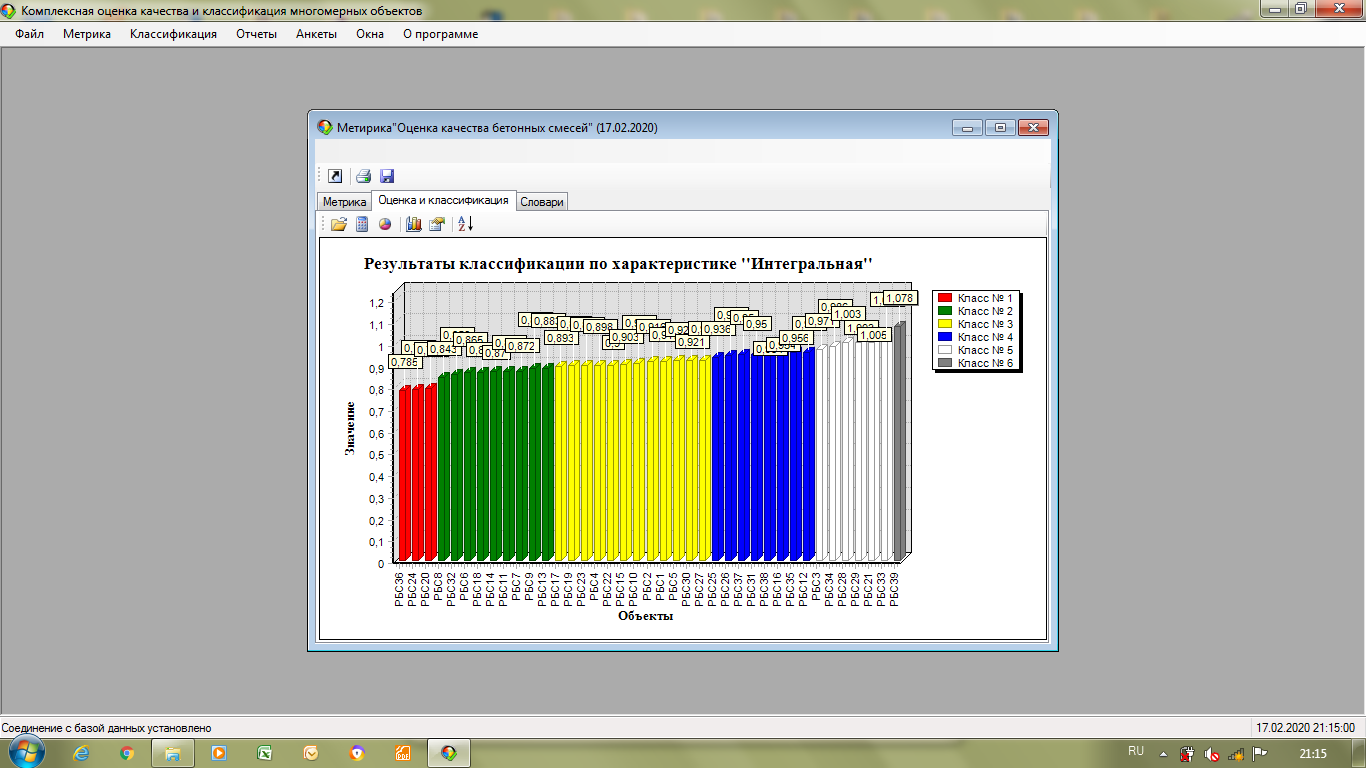
\includegraphics[width=0.8\textwidth]{image10}
  \caption*{Fig. 3- Clustering of concrete mix formulations}
\end{figure}

\begin{longtable}[]{@{}
  |>{\raggedright\arraybackslash}p{(\columnwidth - 10\tabcolsep) * \real{0.1486}}|
  >{\raggedright\arraybackslash}p{(\columnwidth - 10\tabcolsep) * \real{0.1629}}|
  >{\raggedright\arraybackslash}p{(\columnwidth - 10\tabcolsep) * \real{0.1812}}|
  >{\raggedright\arraybackslash}p{(\columnwidth - 10\tabcolsep) * \real{0.1449}}|
  >{\raggedright\arraybackslash}p{(\columnwidth - 10\tabcolsep) * \real{0.1631}}|
  >{\raggedright\arraybackslash}p{(\columnwidth - 10\tabcolsep) * \real{0.1992}}|@{}}
\caption*{Table 2. Recipe of cluster 5-6} \\
\toprule\noalign{}
\begin{minipage}[b]{\linewidth}\centering
Cluster №
\end{minipage} & \begin{minipage}[b]{\linewidth}\centering
№ recipes
\end{minipage} & \begin{minipage}[b]{\linewidth}\centering
Ravr.сompr.

Mpa
\end{minipage} & \begin{minipage}[b]{\linewidth}\centering
ash

g/\%
\end{minipage} & \begin{minipage}[b]{\linewidth}\centering
Metall. Slagg/\%
\end{minipage} & \begin{minipage}[b]{\linewidth}\centering
bauxite sludge

g/\%
\end{minipage} \\
\midrule\noalign{}
\endhead
\bottomrule\noalign{}
\endlastfoot
\multirow{6}{*}{5} & RBS3 & 8.32 & & & 674/5 \\
& RBS34 & 8.18 & & & 842/7 \\
& RBS28 & 9 & 337/2.5 & 798/6 & 505/4 \\
& RBS29 & 10 & 337/2.5 & 1596/12 & \\
& RBS33 & 9.1 & 164/1.3 & & 1685/13 \\
& RBS21 & 9.74 & 328/2.5 & 798//6 & 246/2 \\
\hline
6 & RBS39 & 22.3 & 505/4 & 1197/9.2 & 337/2.5 \\
\end{longtable}

{\bfseries Methods and materials}. As a software tool for clustering
concrete mix formulations, we use the DBSCAN clustering algorithm
{[}4-11{]}.

DBSCAN (Density-based spatial clustering of applications with noise), a
density algorithm for spatial clustering with the presence of noise), as
the name implies, operates with data density.

We use the same data as in {[}1{]}.Ideally, DBSCAN can achieve good
results, but it\textquotesingle s not worth hoping for. Many versions of
the algorithm are able to work from cluster to cluster.

At the same time, the algorithm considers clusters as high-density areas
separated by low-density areas.

Because of this, clusters obtained in DBSCAN come in any shape, unlike
k-means, which assume that clusters are convex.

In practice, an important component of DBSCAN is a cluster consisting of
a set of core samples, "each of which is close to each other (measured
using some distance measurement measure) and a set of non-core samples
that are close to the core sample (but are not core samples themselves)"
{[}4{]}.

2 parameters are important for the DBSCAN algorithm: min\_samples and
eps, high min\_samples or lower eps, provide the high density necessary
for cluster organization.

The algorithm is formed in this way:

\begin{enumerate}
\item
All points are marked as core, boundary or noise;

\item
Interference will be eliminated;

\item
The face between all the main points located inside at the distance
of the Eps parameter from each other is marked;

\item
Each group is placed in a separate cluster;

\item
The boundary points of one of the clusters associated with this
boundary point are specified.
\end{enumerate}

At the same time, the base sample is part of a cluster, a sample that is
not a core sample, and exists, at a distance of eps from any core
sample, is considered an anomaly of the algorithm.

The algorithm executed (DensitybasedClusteringAlgorithm) allows the
cluster to grow until the density in the neighboring cluster exceeds a
certain threshold.

The DBSCAN algorithm is deterministic, always generating the same
clusters when providing the same data in the same order. However, the
results may differ if the data is provided in a different order. First,
even though core samples will always be assigned to the same clusters,
the labels of these clusters will depend on the order in which these
samples occur in the data. Secondly, and more importantly, the clusters
to which the non-core samples are assigned may differ depending on the
order of the data.

The clustering algorithm is effective when, as a rule, the "compactness
hypothesis" can be implemented, while splitting objects into classes,
the distances between objects from the same class
(intra-clusterdistances) will be less than some value
ϵ\textgreater0�\textgreater0, and between objects from different classes
(cross-clusterdistance) will be greater than ϵ�.

For our case, a table of distances between classes is formed in Figure 4.

\begin{figure}[H]
\begin{subfigure}[b]{0.5\linewidth}
  \centering
  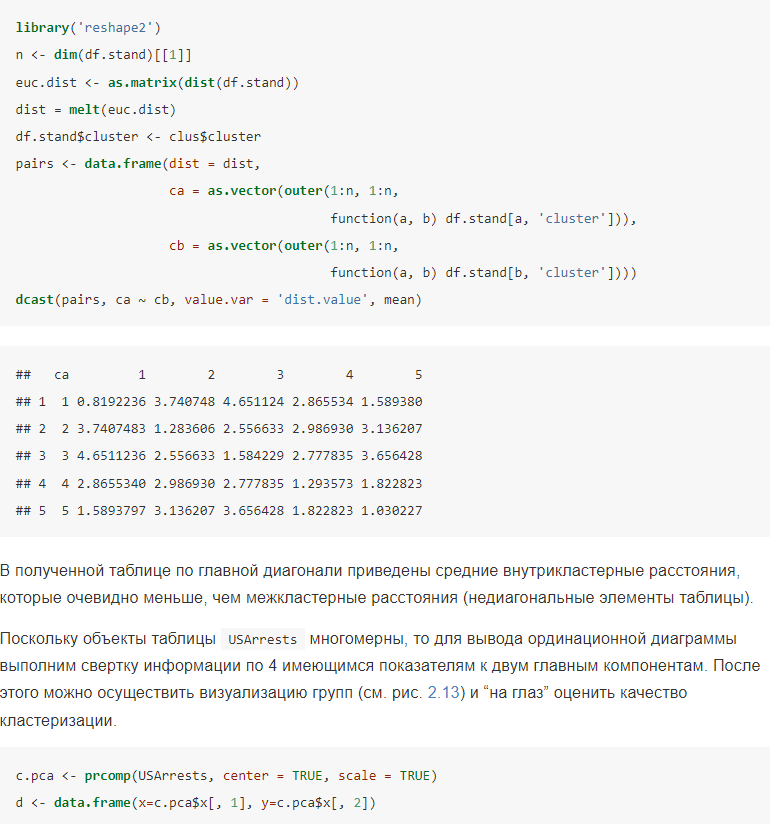
\includegraphics[width=\linewidth]{image77}
  \caption*{Fig. 4 - Table of distances between classes}
\end{subfigure}
\begin{subfigure}[b]{0.5\linewidth}
  \centering
  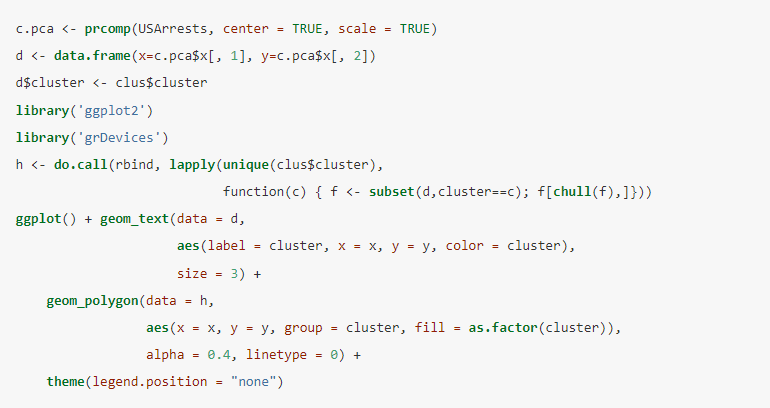
\includegraphics[width=\linewidth]{image78}
  \caption*{Fig. 5 - Dependencies of distances inside and outside clusters}
\end{subfigure}
\end{figure}

From Figure 5, we see that the average intracluster distances are
significantly smaller than the intercluster distances.


As a result, using the DBSCAN algorithm, the distribution of concrete
mix formulations by class is obtained, as shown in Figure 6.

Figure 7 shows the clustering of concrete mix formulations.

\begin{figure}[H]
\begin{subfigure}[b]{0.45\textwidth}
  \centering
  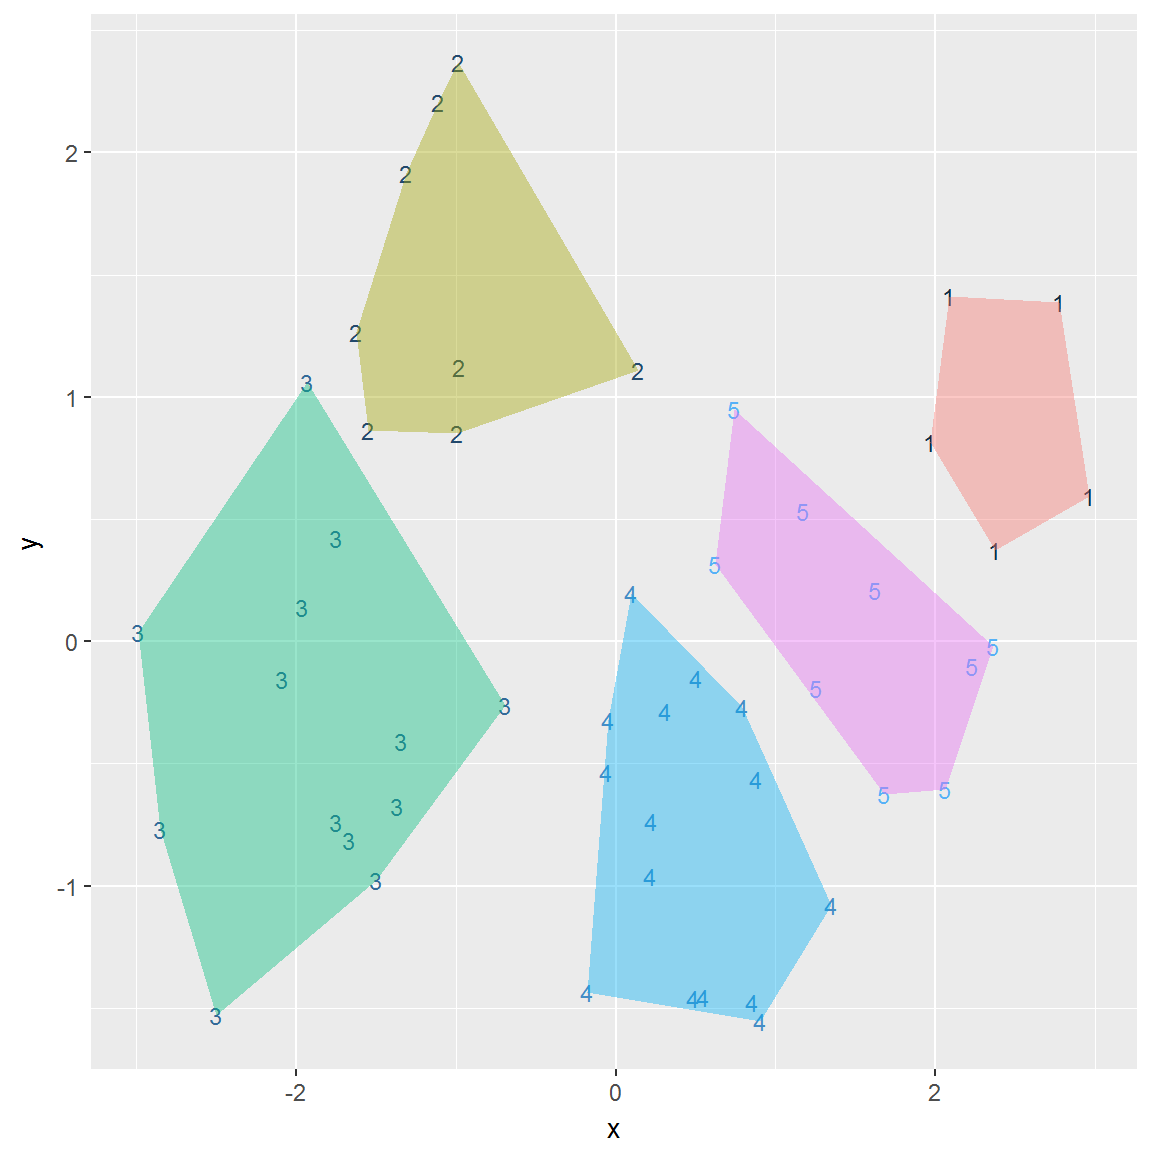
\includegraphics[width=\textwidth]{image13}
  \caption*{Fig. 6 - Results of the distribution of concrete mix recipe by class}
\end{subfigure}
\hspace{0.05\textwidth}
\begin{subfigure}[b]{0.45\textwidth}
  \centering
  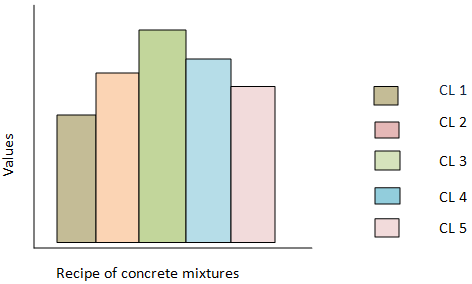
\includegraphics[width=\textwidth]{image14}
  \caption*{Fig. 7 - Distribution of concrete mix formulations by clusters}
\end{subfigure}
\end{figure}

\begin{multicols}{2}
{\bfseries Discussion and results}. As can be seen from Figure 7, all the
formulations of concrete mixtures are combined into 5 clusters. The
largest is cluster 3, the smallest is cluster 1.

The task of describing in detail which formulations of concrete mixtures
were included in each cluster was not set.

Clustering technology using datamining is quite complex, the difficulty
lies in the uncontrolled decision-making process. It is not completely
clear whether the correct solution has been achieved.

"Deep artificial neural networks are very good at classification, but
clustering is still an open question"{[}2{]}.

{\bfseries Conclusions.} We see that DataMining is quite a promising tool
for clustering, including formulations of concrete mixtures. Although
the results leave much to be desired compared to those previously
obtained in {[}1{]}, nevertheless, with fairly constant machine learning
and training, there is a potential prospect that we will get good
clustering results. In the future, we plan to use one of the software
tools presented above for clustering man-made waste of the Pavlodar
region.
\end{multicols}

\begin{center}
{\bfseries Referenses}
\end{center}

\begin{enumerate}
\item
Akishev K and other. Mathematical formulation and the problem
solution of clustering recipes of concrete mixtures using technogenic
waste waste and slags of metallurgical enterprises.- Метаllurjia. -
2022. - 61(1)213-216. Zagreb, p.321.

\item
Electronicresource URL: \href{https://trends.rbc.ru/trends/amp/news/61b359739a7947c7376ef7ce/}{https://trends.rbc.ru} -Date of application 12.05.2023.

\item
Electronic resource:URL: \href{https://cyberleninka.ru/article/n/analiz-i-klassifikatsiya-algoritmov-klasterizatsii}{https://cyberleninka.ru} - Date of application 12.05.2023.

\item
Electronic resource: URL:\href{https://etu.ru/assets/files/nauka/dissertacii/2009/SIElizarov.doc}{https://etu.ru}. -date of application 12.05.2023.

\item
Electronic resource: URL:\href{https://elibrary.ru/item.asp?id=45420956}{https://elibrary.ru} - Date of application
12.05.2023.

\item
Electronic resource: URL:\href{https://habr.com/ru/articles/322034/}{https://habr.com} -Date of application 12.05.2023.

\item
Electronic resource:URL:
\href{http://pzs.dstu.dp.ua/DataMining/cluster/bibl/\%25D0\%9A\%D0\%9B\%D0\%90\%D0\%A1\%D0\%A2\%D0\%95\%D0\%A0\%D0\%98\%D0\%97\%D0\%90\%D0\%A6\%D0\%98\%D0\%AF\%20\%D0\%9E\%D0\%91\%D0\%AA\%D0\%95\%D0\%9A\%D0\%A2\%D0\%9E\%D0\%92\%20\%D0\%A1\%20\%D0\%9F\%D0\%9E\%D0\%9C\%D0\%9E\%D0\%A9\%D0\%AC\%D0\%AE\%20\%D0\%90\%D0\%9B\%D0\%93\%D0\%9E\%D0\%A0\%D0\%98\%D0\%A2\%D0\%9C\%D0\%90\%20DBSCAN.pdf}{http://pzs.dstu.dp.ua/DataMining}
- Date of application 12.05.2023.

\item
Electronicresource: URL: \href{https://www.math.spbu.ru/SD_AIS/documents/2014-05-341/2014-05-tw11.pdf}{https://www.math.spbu.ru}
-Date of application 12.05.2023.

\item
Electronicresource:URL: \href{https://core.ac.uk/download/pdf/196226625.pdf}{https://core.ac.uk} - date of
application 12.05.2023.

\item
Electronic resource :URL: Ortiz-Arroyo D. Discovering Sets of Key
Players in Social Networks // Computational Social Networks Analysis. -
2010 - C. 27-47 {[}Date of application 12.05.2023.

\item
Electronic resource:URL:
\href{https://kpfu.ru/portal/docs/F_1980845423/161_3\%20_phys\%20_mat_8.pdf}{https://kpfu.ru/portal/docs/F\_1980845423/161\_3\_phys\_mat\_8.pdf} - Date of application 12.05.2023.
\end{enumerate}

\emph{{\bfseries Information about the authors}}

\begin{itemize}
\item
Akishev Karshyga Maksutovich, Candidate of Technical Sciences, Ass.
Professor, Department of "Information Technology", Kazakh University of
Technology and Business, Astana, Republic of
Kazakhstan

email:akmail04cx@mail.ru

\item
Karpov Valery Ivanovich, Doctor of Technical Sciences, Professor,
Department of Information Technology, Moscow State University of
Technology and Management named after K.G. Razumovsky, Moscow, Russia
email:Vikarp@mail.ru

\item
Akisheva Lenara Karshygaevna, 7th grade student of Nazarbayev
Intellectual School, Astana, Republic of Kazakhstan email:LK@mail.ru

\item
Tulegulov Amandos Dabysovich, Ph.D., Ass. Professor, Head of the
Department of "Information Technology", Kazakh University of Technology
and Business, Astana, Republic of Kazakhstan email:tud62@yandex.ru
\end{itemize}

\emph{{\bfseries Сведения об авторах}}

\begin{itemize}
\item
Акишев Каршыга Максутович, к.т.н., асс. профессор, кафедра
«Информационные технологии», Казахский университет технологии и бизнеса,
г. Астана, Республика Казахстан: email:akmail04cx@mail.ru

\item
Карпов Валерий Иванович, доктор технических наук, профессор, кафедра
«Информационные технологии» Московский Государственный универститет
технологии и управления имени К.Г. Разумовского,г. Москва,
Россия:email:Vikarp@mail.ru

\item
Акишева Ленара Каршыгаевна, ученица 7 классса Назарбаев Интеллектуальная
школа, г. Астана, Республика Казахстан LK@mail.ru

\item
Тулегулов Амандос Дабысович, к.ф.м.н., асс. профессор, зав. кафедрой
«Информационные технологии», Казахский университет технологии и бизнеса,
г. Астана, Республика Казахстан: tud62@yandex.ru
\end{itemize}
